\documentclass[11pt,a4paper]{ctexart}
\usepackage[margin=2cm]{geometry}
\usepackage{amsmath,amssymb,bm}
\usepackage{booktabs,graphicx,xcolor,hyperref,array,float,multicol}
\hypersetup{colorlinks=true,linkcolor=blue,urlcolor=blue}
\setlength{\parindent}{2em}
\setlength{\parskip}{0.25em}
\setlength{\emergencystretch}{3em}
\title{InEKF 机载实现评估：Numba、Cython、CUDA 与 C++}
\author{基于当前 15 维右不变滤波核的实测与结构分析}
\date{2026年7月24日}

\begin{document}
\maketitle

\section{结论}

对当前单飞行器、单 InEKF、在线逐事件处理的任务，不建议将 CPU Numba 核迁移到
Numba-CUDA。预计固定尺寸 C++ CPU 最快；彻底静态类型化的 Cython 与 CPU Numba
处于同一高性能等级；CUDA 对该单实例小矩阵递推通常无优势且可能增加延迟；
无 Numba 的 Python/NumPy 最慢。

实飞适用性排序为：生产级固定尺寸 C++ 最优；深度 Cython 可作为 Linux companion
computer 的 AOT 过渡；CPU Numba 适合科研实飞和快速验证；纯 Python 适合作为
参考实现；Numba-CUDA 不应成为当前滤波热路径。这里 C++、Cython 与 CUDA 的排序
是结构分析结论，不是未做实验却虚构出的倍数。

\section{与论文递推的关系}

论文和当前实现维护 15 维误差状态
\begin{equation}
 \delta x_k=
 [\delta\theta_k,\delta v_k,\delta p_k,\delta b_{g,k},\delta b_{a,k}]
 \in\mathbb{R}^{15},
\end{equation}
并执行
\begin{align}
 \hat X_{k+1}^{-}&=f(\hat X_k^{+},u_k,\Delta t_k),\\
 P_{k+1}^{-}&=\Phi_kP_k^{+}\Phi_k^{\mathsf T}+Q_{d,k},\\
 S_j&=H_jP_j^-H_j^{\mathsf T}+R_j,\\
 \delta x_j&=P_j^-H_j^{\mathsf T}S_j^{-1}r_j,\\
 P_j^+&=P_j^--\frac{u_ju_j^{\mathsf T}}{S_j},
 \qquad u_j=P_j^-H_j^{\mathsf T}.
\end{align}
当前 Numba 改变的是上述公式的执行方式，不改变状态维数、float64、事件顺序、
噪声、NIS 门限或状态注入。

\section{CUDA 并行度上限}

令完整滤波状态为
\begin{equation}
 z_k=(\hat X_k,P_k,b_k).
\end{equation}
在线事件递推是有向链
\begin{equation}
 \boxed{z_{k+1}=\mathcal F_k(z_k,u_k,y_k)}.
\end{equation}
因此 $z_{k+2}$ 必须等待 $z_{k+1}$，相邻 IMU/UWB 时间步不能分派给独立 CUDA
线程并行执行。GPU 只能在单步内部并行小矩阵元素，最大矩阵为 $15\times15$，
UWB 又是标量秩一更新；这种计算粒度不足以掩盖 kernel launch、同步和访存开销。

若每个事件启动 $m$ 个小 kernel，总延迟可写成
\begin{equation}
 T_{\mathrm{GPU,event}}
 =mT_{\mathrm{launch}}+T_{\mathrm{sync}}+
 T_{\mathrm{memory}}+T_{\mathrm{compute}},
\end{equation}
而 CPU Numba 已把完整事件平均压到约 $6.1$--$6.4~\mu s$。若把整条递推放入一个
persistent kernel，启动项可以摊薄，但只有一个小线程块沿时间轴前进，其余 SM
仍处于低占用状态。

\section{数据集实测}

三组 AB/BA 配对测试固定数值库为单线程；计时包含完整状态、旋转、$15\times15$
协方差、偏置和 NIS 历史。JIT 缓存加载/预热为 $0.3004$ s，单独记录。

\begin{table}[H]
\centering
\small
\caption{当前工作站 CPU 实测；CUDA 与 C++ 未实现，未伪造计时}
\begin{tabular}{p{3.7cm}rrrr}
\toprule
数据 & Python [s] & Numba [s] & 加速 & Numba/数据时长\\
\midrule
const1, yaw $0^\circ$, 30 s & 4.5567 & 0.2706 & 16.84$\times$ & 0.902\%\\
const4, yaw $90^\circ$, 60 s & 9.3616 & 0.5269 & 17.77$\times$ & 0.878\%\\
const3, yaw $180^\circ$, 60 s & 7.9309 & 0.4751 & 16.69$\times$ & 0.792\%\\
\bottomrule
\end{tabular}
\end{table}

令实时计算负载比为
\begin{equation}
 \rho=\frac{T_{\mathrm{compute}}}{T_{\mathrm{data}}}.
\end{equation}
当前 Numba 的 $\rho=0.792\%$--$0.902\%$，即完整历史模式下仍有约
$111$--$126$ 倍实时余量；无 Numba 路径为 $13.2\%$--$15.6\%$。两种路径的
四项 RMSE 相对差小于约 $10^{-10}\%$，UWB 拒绝决策变化为零。

\begin{figure}[H]
\centering
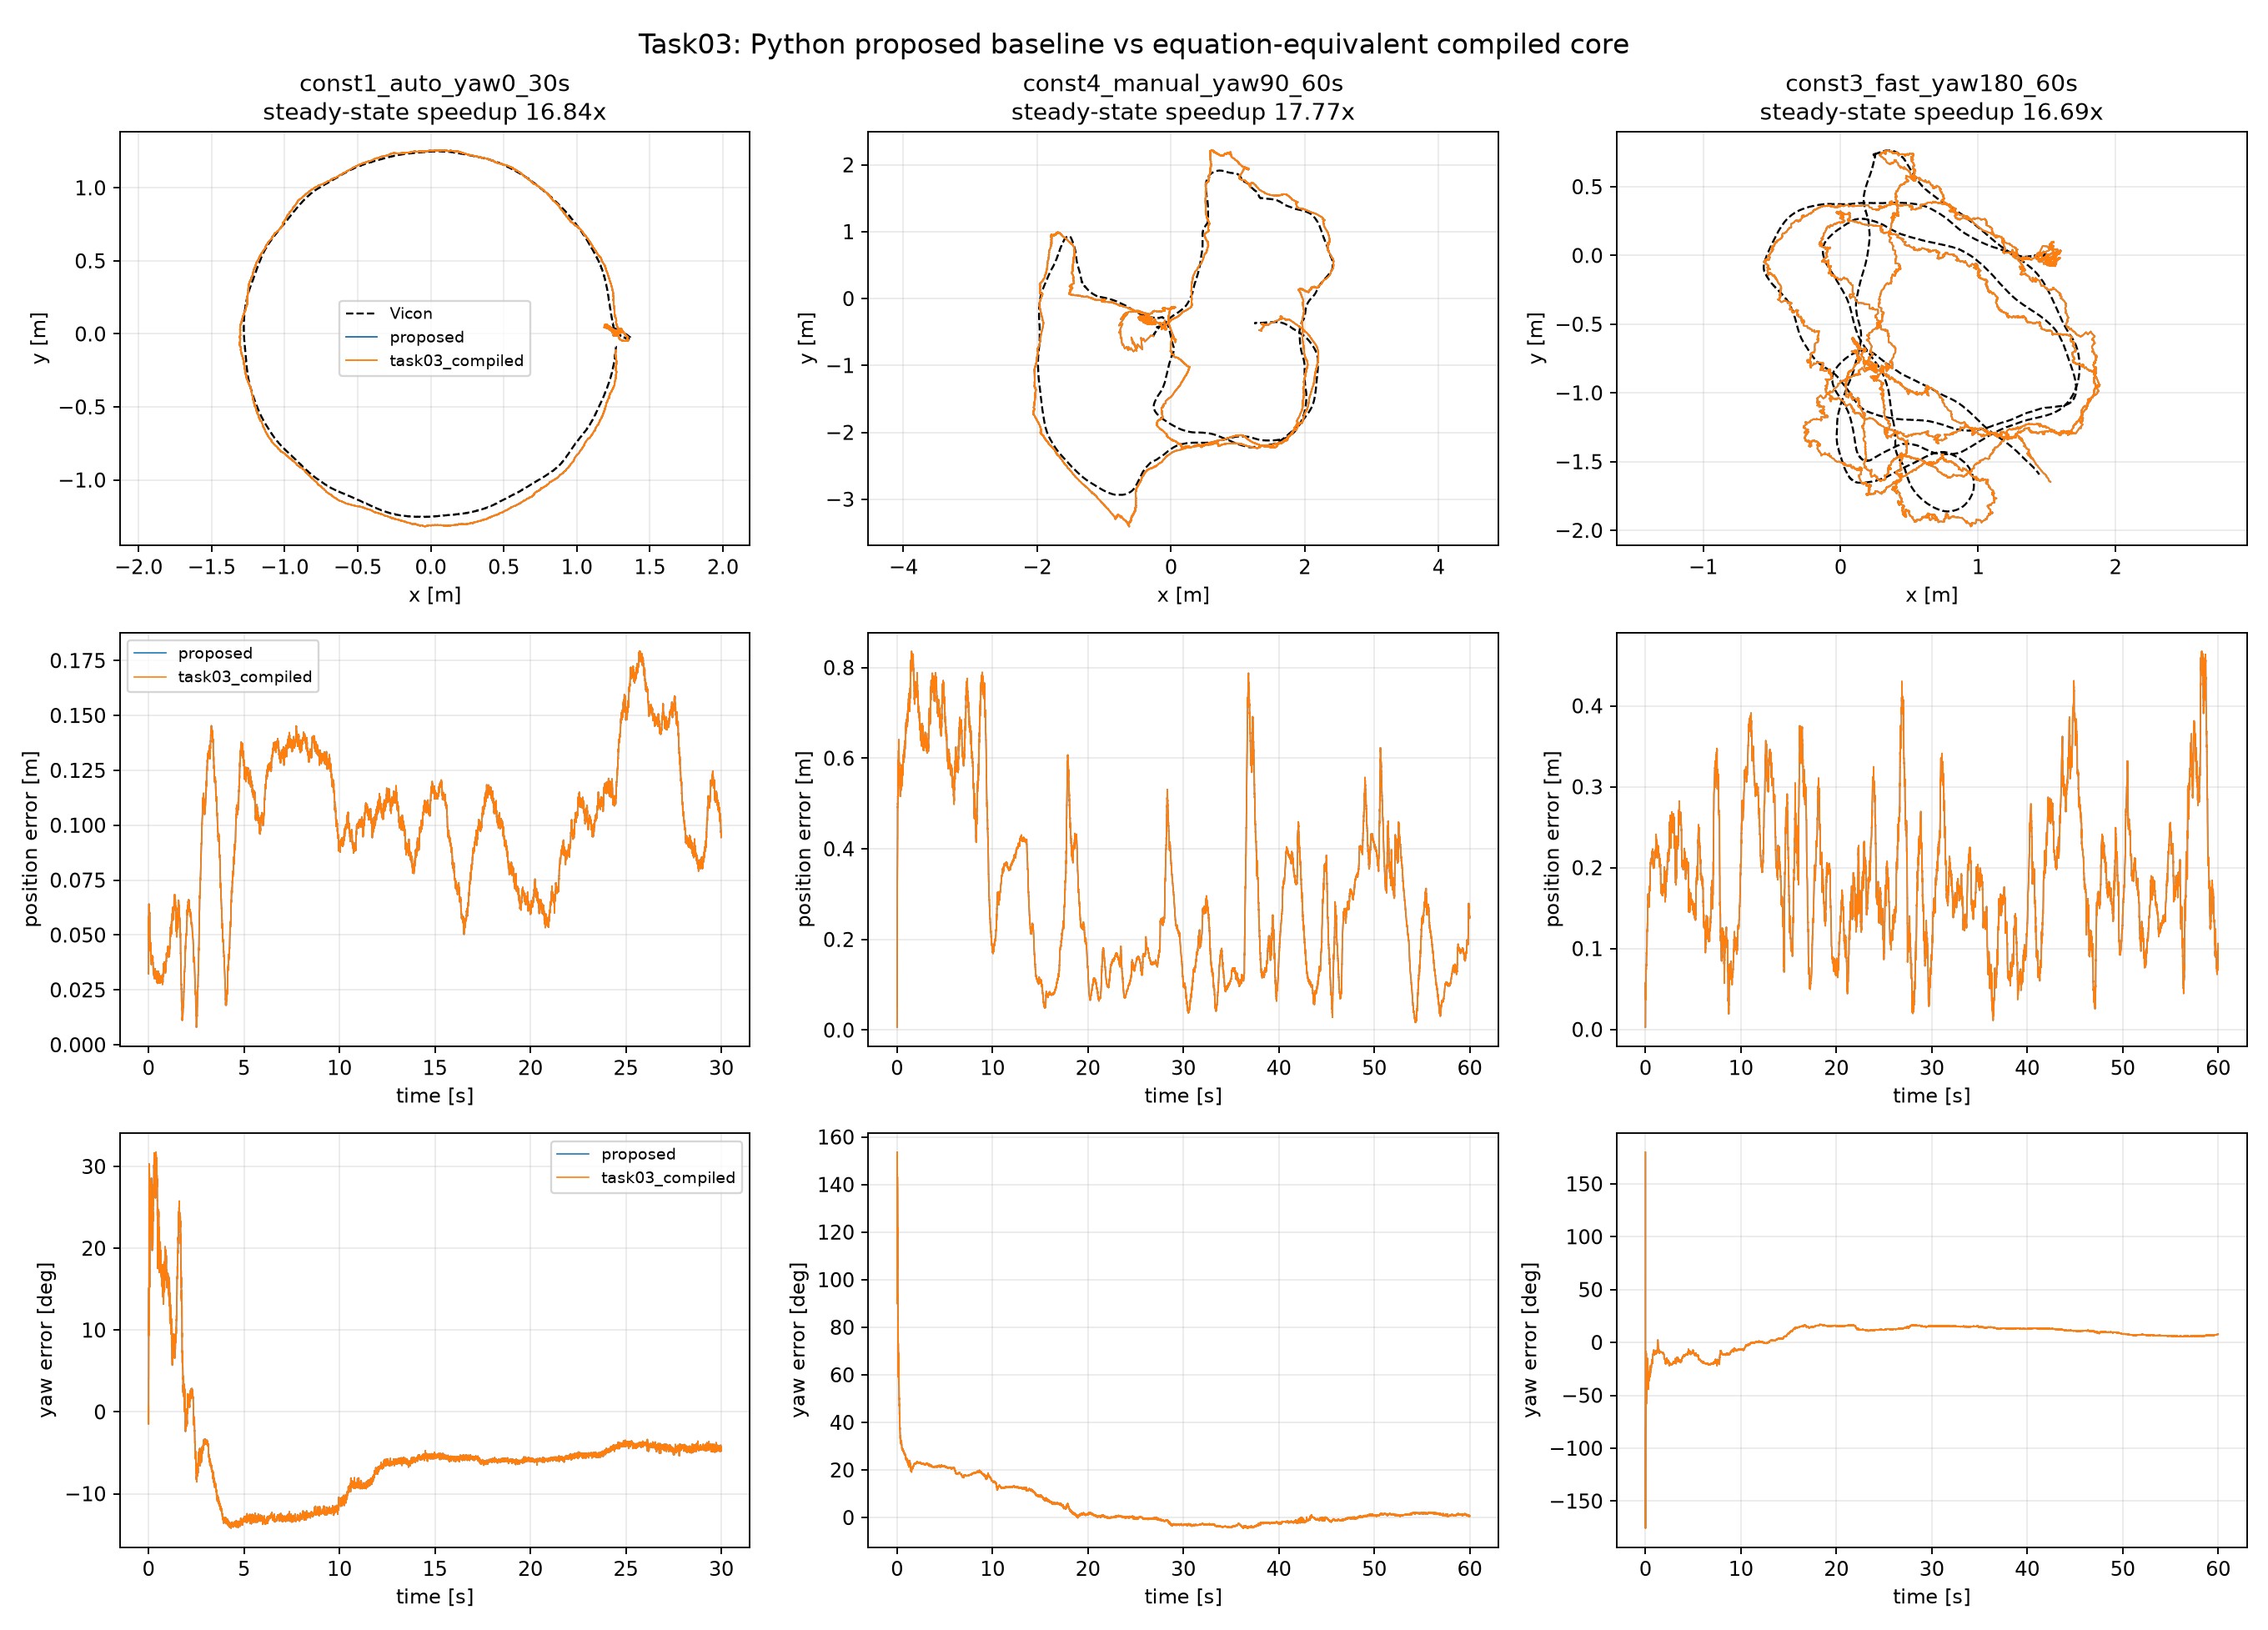
\includegraphics[width=\textwidth]{../imu-uwb-inekf/results/cuda_feasibility_cpu_baseline_2026-07-24/comparison.png}
\caption{CPU Numba 与无 Numba 的轨迹、位置误差和 yaw 误差。两条估计曲线逐点
重合；const3 收敛后的 yaw 偏差是已有算法现象，不是编译引入。}
\end{figure}

\section{方案比较}

\begin{table}[H]
\centering
\small
\caption{当前单滤波器在线任务的工程排序}
\begin{tabular}{p{2.5cm}p{3.0cm}p{3.5cm}p{4.7cm}}
\toprule
方案 & 速度结论 & 部署特征 & 实飞判断\\
\midrule
Python/NumPy & 已实测最慢 & Python 调度和临时分配较多 & 仅参考、回放和原型\\
CPU Numba & 已实测快 16.69--17.77 倍 & 需 Python/LLVM、预热和缓存管理 &
科研实飞推荐，短期保留\\
深度 Cython & 未实测；预计与 Numba 同量级 & AOT，无 JIT；依赖 CPython ABI &
AOT 过渡方案\\
Numba-CUDA & 未实测；预计单实例无优势 & GPU/驱动/CUDA 版本绑定，资源竞争复杂 &
当前不推荐\\
固定尺寸 C++ & 未实测；预计最快或与 Numba 同量级 & 可静态分配、控制线程与异常 &
生产实飞首选\\
\bottomrule
\end{tabular}
\end{table}

当前 CPU 核使用设备代码不支持的动态数组创建、矩阵表达式和线性代数接口，因此
CUDA 版本不是把 \texttt{@njit} 替换成 \texttt{@cuda.jit}，而要重写固定索引、
共享内存、同步和小矩阵运算。统一内存的 Jetson 可减少 PCIe 拷贝，但不会改变
式 (7) 的时间串行依赖。

\section{Cython 对结论的影响}

Cython 必须区分两个层次。浅层做法只是把现有文件编译为扩展，却继续调用
\texttt{np.zeros}、\texttt{@}、\texttt{np.outer} 和 Python/NumPy 对象；它只减少
少量分派，不会自动达到 Numba 速度。深度做法则将状态、协方差和临时量写成连续
\texttt{double} typed memoryview 或固定 C 数组，以固定循环实现 $3\times3$ 和
$15\times15$ 运算，热路径不创建 Python 对象，并明确使用
\texttt{cdef inline}、\texttt{noexcept} 与合适的 \texttt{nogil} 边界。这种实现
才可能与 Numba/C++ 同量级，但工作量已接近一次受控 C/C++ 移植。

Cython 在构建期生成 C/C++ 并编译为 \texttt{.so}/\texttt{.pyd}，因此没有 Numba
首次 JIT 或缓存加载延迟。它仍依赖 CPython 解释器和目标平台扩展 ABI，不等同于
独立 C++ 二进制。官方还明确说明，释放 GIL 不会让同一份单线程 C 级代码本身更快；
它的价值是允许 I/O/传感器线程并发。当前相邻滤波时间步仍严格串行，所以 Cython
不改变 CUDA 并行度结论。

当前项目环境未安装 Cython，本轮没有实现 Cython 核，也没有伪造倍数。因此更新后的
单实例预测为
\begin{equation}
 \boxed{\text{固定尺寸 C++}\ \gtrsim\
 \{\text{深度 Cython},\ \text{CPU Numba}\}
 \ \gg\ \text{无 Numba Python}.}
\end{equation}
深度 Cython 和 Numba 谁略快只能在相同计时边界和目标机载硬件上决定。

\section{适用边界与建议}

CUDA 只有在存在大量独立实例时才值得重新评估，例如几十到几百个滤波器、粒子、
多 yaw 假设、Monte Carlo 或离线全数据集批处理。此时合理映射是每个独立实例使用
一个 warp/block，而不是并行同一滤波器的相邻时间步。

近期实飞保持 CPU Numba，关闭无必要的完整历史，启动时强制预热和自检。若希望先
消除 JIT，可将深度 Cython AOT 核设为中间里程碑；若热循环仍调用 NumPy 或目标是
MCU，应直接转固定尺寸 C++。所有候选实现都要用全部 79 个 CSV 对状态、协方差、
NIS、拒绝决策和 RMSE 做跨语言 golden regression。最终必须在选定机载计算机上测试
p50/p95/p99/max 单事件时延、长时间热降频、内存、传感器 I/O 干扰和 GPU 满载
竞争，不能用桌面平均回放代替目标硬件 WCET。

\section{资料}

\begin{multicols}{2}
\small
\begin{itemize}
\setlength{\itemsep}{0.15em}
 \item \href{https://numba.readthedocs.io/en/0.61.0rc1/reference/deprecation.html}
 {Numba 内置 CUDA target 弃用说明}
 \item \href{https://nvidia.github.io/numba-cuda/user/installation.html}
 {Numba-CUDA 安装与版本支持}
 \item \href{https://nvidia.github.io/numba-cuda/}
 {Numba-CUDA 维护状态}
 \item \href{https://nvidia.github.io/numba-cuda/user/cudapysupported.html}
 {CUDA Python 支持的 Python/NumPy 子集}
 \item \href{https://www.nvidia.com/en-eu/autonomous-machines/embedded-systems/jetson-orin/}
 {NVIDIA Jetson Orin 官方规格}
 \item \href{https://cython.readthedocs.io/en/stable/src/userguide/source_files_and_compilation.html}
 {Cython 源码与 AOT 扩展编译}
 \item \href{https://cython.readthedocs.io/en/latest/src/userguide/numpy_tutorial.html}
 {Cython 的 NumPy 类型化性能路径}
 \item \href{https://cython.readthedocs.io/en/latest/src/userguide/nogil.html}
 {Cython nogil 的作用与限制}
\end{itemize}
\end{multicols}

\end{document}
